% !TEX root = ../dissertation.tex

\chapter{Low Thrust Orbital Transfers using Reachability Sets}\label{sec:lowthrust_transfers}
In this chapter, we propose a systematic design method which enables low-thrust transfers in the planar circular restricted three-body problem as well as an extension for use about asteroids.
We utilize the concept of the reachability set to enable a simple methodology of selecting initial conditions to achieve general orbital transfers. 
The reachable set, defined as the set of all attainable states subject to the system constraints, allows for the extension of the previous control-free methods based on invariant manifolds.
Defining the reachable set on a \Poincare section reduces the dimensionality of the system dynamics to the study of a related discrete update map.
Through the use of low-thrust control input, the reachable set on the \Poincare section is enlarged and enables a larger space of potential transfers.
By iteratively computing the reachable set, and minimizing the distance to the target on the \Poincare section, we generate general transfer trajectories.
With this proposed method, the previous research on control-free trajectories will be generalized with the addition of low thrust propulsion systems.

The method is formulated as an extension to the control free method based on invariant manifolds in the three-body problem~\cite{koon2011}.
Much of the previous work using invariant manifolds has been applied to the planar circular restricted three body problem.
This paper provides a discrete optimal control formulation to generate the reachability set on a \Poincare section.

\section{Planar Circular Restricted Three Body Problem}\label{sec:pcrtbp}
% discuss some of the pros/cons of using PCRTBP model
We utilize the \gls{pcrtbp} as the basis of our system definition. 
It is a popular model in the preliminary analysis of multibody spacecraft trajectories. 
In the context of Earth based mission, the \gls{pcrtbp} affords a relatively simple dynamic model while still capturing the major third body perturbation of the Moon.
In addition, this model allows for a systematic process to define and exploit \Poincare sections.
Furthermore, the 2D solutions afforded by the \gls{pcrtbp} are frequently used to gain a qualitative understanding of the trade space of transfers in the Earth-Moon system.
The PCRTBP approach offers insight into the fundamental dynamical structure while capturing the major dynamic properties of the planar motion.
As a result, this approach is best suited for preliminary trajectories which do not require large plane changes.

The Earth is assumed to be the more massive primary, \( m_1 \), while the Moon is the second, smaller primary \( m_2\).
The equations of motion are developed in a rotating reference frame which allows for much greater insight into the structure of the dynamics.
This rotating reference frame is later used when deriving the motion about an asteroid.
Following convention, the system is also non-dimensionalized by the characteristic units of length, mass, and time~\cite{koon2011}.
As a result, the system can be characterized by a single mass ratio parameter \( \mu \),
\begin{equation}
        \mu = \frac{m_2}{m_1+m_2} \, .
        \label{eq:mass_param}
\end{equation}
In the rotating reference frame the Lagrangian is given by
\begin{equation}\label{eq:pcrtb_lagrangian}
    L = \frac{1}{2} \parenth{\parenth{\dot{x} - y}^2 + \parenth{\dot{y} + x}^2} + \frac{1 - \mu}{r_1} + \frac{\mu}{r_2},
\end{equation}
where the distances \( r_1, r_2 \in \R \) define the distance from the spacecraft to each primary and are defined as
\begin{align}
    r_1 &= \sqrt{\parenth{x + \mu}^2 + y^2} , \\
    r_2 &= \sqrt{\parenth{x -1 + \mu}^2 + y^2} .
\end{align}
Following a straightforward application of the Euler-Lagrange equations, a more detailed derivation is provided in~\cite{szebehely1967}, results in the following equations of motion defined in the rotating reference frame
\begin{equation}\label{eqn:cont_dyn}
        \left[\begin{array}{c} \dot{\vc{r}} \\ \dot{\vc{v}} \end{array} \right] = 
        \left[ \begin{array}{c} \vc{v} \\ A \vc{v} + \nabla U + \vc{u} \end{array} \right] = f\left( t,\vc{x}, \vc{u}\right) \, ,
\end{equation}
where the matrix \( A \) and pseudo gravitational potential gradient \( \nabla U\) are
\begin{align}
    A &= \left[ \begin{array}{ccc} 0 & 2 & 0 \\ -2 & 0 & 0 \\ 0 & 0 & 0 \end{array} \right], \label{eq:A_mat} \\
    \nabla U &= \left[ \begin{array}{c} x - \frac{ \left(1 - \mu\right) \left(x + \mu\right)}{r_1^3} - \frac{\mu \left( x - 1 + \mu \right)}{r_2^3} \\
                                                                                        y - \frac{ \left(1 - \mu\right) y}{r_1^3} - \frac{\mu y}{r_2^3} \\
                                                                                        - \frac{ \left(1 - \mu\right) z}{r_1^3} - \frac{\mu z}{r_2^3}\end{array}\right]
                                        = \left[\begin{array}{c} U_x \\ U_y \\ U_z\end{array} \right] , \label{eq:grav_pot}
\end{align}
and the control input is defined as \( \vc{u} = \begin{bmatrix} u_x & u_y \end{bmatrix}^T \in \R^{2\times1} \) and assumed to be continuously variable but bounded in magnitude, i.e. \( \vc{u}^T \vc{u} \leq u_{max}^2 \).
The state is defined as \( \vc{x} = \begin{bmatrix}\vc{r} &\vc{v} \end{bmatrix}^T\) with \(\vc{r} = \begin{bmatrix} x & y \end{bmatrix}^T \in \R^{2\times1}\) and \(\vc{v}= \begin{bmatrix} \dot{x} & \dot{y} \end{bmatrix}^T \in \R^{2\times1}\) representing the position and velocity with respect to the system barycenter, respectively.

\subsection{Jacobi Integral}\label{sec:jacobi}
There exists a single integral, or constant of motion for the three-body problem~\cite{szebehely1967,lanczos1970}.
This energy constant is analogous to the total mechanical energy, however it is a non-physical quantity arising from the problem formulation~\cite{szebehely1967}.
Also known as the Jacobi constant, it is defined as a function of the position and velocity in the rotating frame and given by
\begin{equation}
        E\left( \vc{r} , \vc{v} \right) = \frac{1}{2}\left( \dot{x}^2 + \dot{y}^2\right) - U\left(x,y \right) \, .
        \label{eq:jacobi}
\end{equation}
\Cref{eq:jacobi} divides the phase space into distinct regions of allowable motion based on the energy level of the spacecraft.
Fixing the Jacobi integral to a constant defines zero velocity curves, which are the locus of points where the kinetic energy, and hence velocity vanishes.
As seen in Figure~\ref{fig:energy_contour}, the phase space is divided into distinct realms based on the energy level.
In the vicinity of \( m_1\) or \(m_2\) there exists a potential well. 
As the energy level increases there are five critical points of the effective potential where the slope is zero.
Three collinear saddle points on the \(\hat{e}_1\) axis and two equilateral points.
These equilibrium, or Lagrange points, are labeled \( L_i, i = 1, \hdots, 5 \) and are shown in Figure~\ref{fig:energy_contour}.
The Jacobi integral is a valuable invariant property of the three-body system that allows for greater insight into the motion of the spacecraft.
\begin{figure}[htbp]
        \centering
        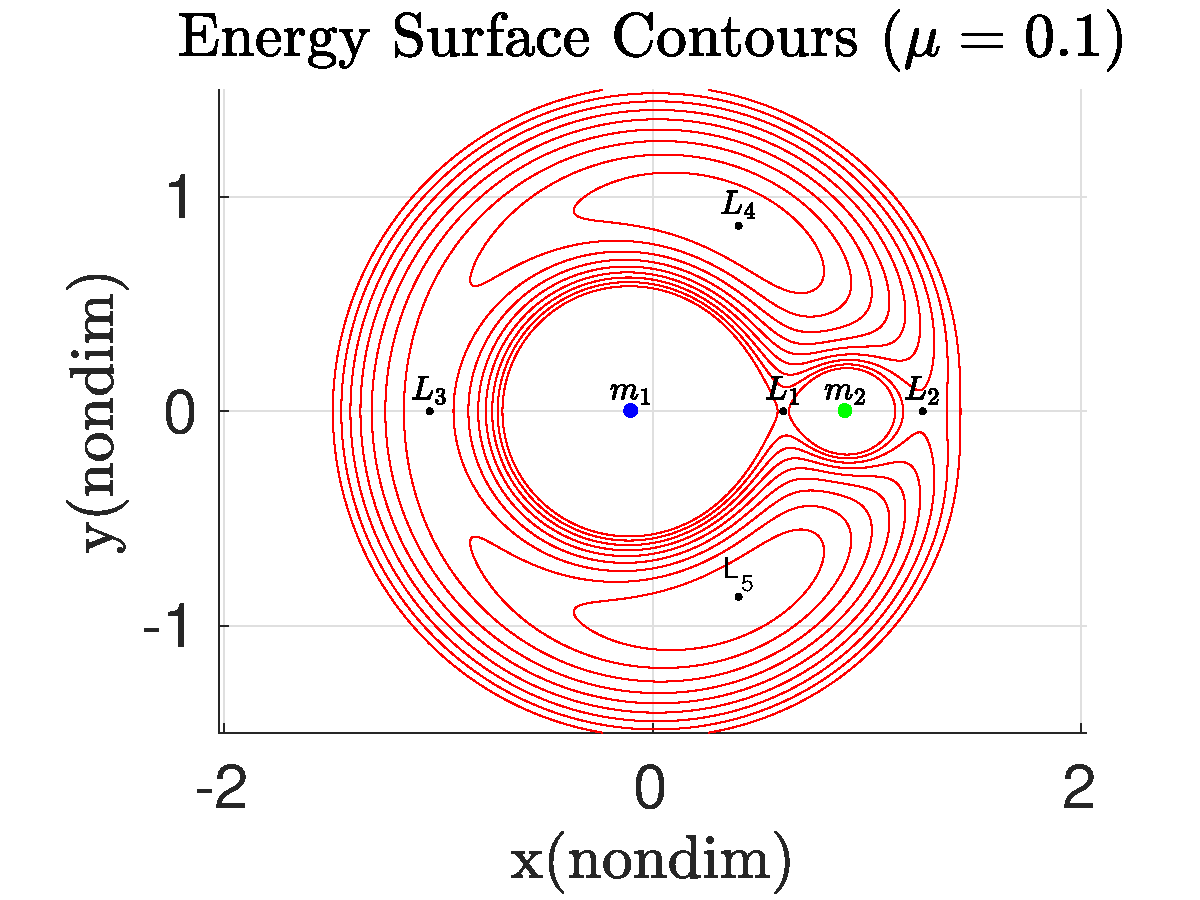
\includegraphics[width=0.75\textwidth]{./figures/2017_JAS/energy_contours.pdf}
        \caption[Jacobi integral]{Contour plot of Jacobi integral: Zero velocity curves of constant Jacobi integral. A particle with fixed energy level cannot cross the contour lines and is therefore limited to specific regions of the phase space. }
        \label{fig:energy_contour}
\end{figure} 

\subsubsection{Invariant Manifolds and \Poincare Map}\label{sec:invariant_manifold}
Dynamics systems theory has been applied to the design of control-free maneuvers in the restricted three-body problem~\cite{koon2011}.
As previously introduced in~\Cref{sec:jacobi}, there exist five equilibrium points in the equations of motion for the three-body problem.
It has been shown that the local orbit structure near the Lagrange points gives rise to families of periodic orbits as well as the stable and unstable manifolds of these periodic orbits.
This rich structure is globally connected and gives rise to a dynamical chain which allows trajectories to pass through the phase space~\cite{koon2011,conley1968}.
The manifold structure associated with periodic orbits about the \( L_1 \) and \( L_2 \) Lagrange points are critical to the understanding of the motion of spacecraft as well as comets/asteroids.
In addition, the stable and unstable manifolds serve as the boundaries of the phase space region that allow for the transport between realms in a single three-body system or between multiple three-body systems.
These invariant manifolds only exist as a result of the dynamic formulation of the three-body problem in a rotating reference frame. 
Invariant manifolds serve as a higher dimensional generalization of the concept of seperatrices from linear systems as applied to the case of nonlinear systems. 

\Poincare maps are a useful tool in the analysis of the flow near periodic orbits in the three-body problem.
We let \( \Sigma \) define a hypersurface of section chosen such that all trajectories in the vicinity of a state \( \vc{q} \in \Sigma \) cross \( \Sigma \) transversely and in the same direction.
A \Poincare map, \( P(\vc{q}) = \phi(T;\vc{q}) \), maps the state of a trajectory from one intersection to the next.
Choosing a section in this manner results in a \Poincare section as shown in~\cref{fig:poincare_map}.
In~\cref{fig:poincare_map} we show two examples of periodic trajectories intersecting the \Poincare section. 
Periodic solutions will appear as fixed points on the section, such as \( q_0, q_1 \) in~\cref{fig:poincare_map}, while stable or unstable trajectories become clearly visible by viewing successive intersections of the section.
This allows for greater insight into the stability and dynamics of periodic solutions of a dynamic system as a fixed point on the \Poincare section corresponds to a periodic orbit while movement on the section is associate with the stability of neighboring trajectories. 
For example, \Poincare maps have been used to prove the existence of homoclinic orbits, which are orbits both forward and backward asymptotic to a single unstable periodic orbit, and heteroclinic orbits, which join different periodic orbits~\cite{conley1968,koon2000b}.
These dynamic features have been shown to play a vital role in the movement of natural bodies as well as critical for spacecraft missions~\cite{gomez2001,lo1997}.
\begin{figure}
        \centering
        \begin{scaletikzpicturetowidth}{0.5\textwidth}
            \tdplotsetmaincoords{60}{125} % view angle in spherical coordinates
    \begin{tikzpicture}[tdplot_main_coords,
      poincare/.style={opacity=.2,very thick,fill=blue},
      orbit/.style={very thick,black},
      orbit hidden/.style={very thick,dashed},
      grid/.style={very thin,gray!50},
      axis/.style={->,blue,thick}, scale=\tikzscale]

    % nodes for the poincare section
    \node[label=above:\(\Sigma\)] (upper_right) at (0,5,5) {};
    \node[] (upper_left) at (0,1,5) {};
    \node[] (lower_left) at (0,1,0) {};
    \node[] (lower_right) at (0,5,0) {};

    % draw poincare section
    \draw[poincare] (upper_right.center) -- (upper_left.center) -- (lower_left.center) -- (lower_right.center) -- (upper_right.center);
    
    % draw a periodic orbit
    \coordinate (center) at (0,0,2);
    \node[below right] (x0) at (0,2,2) {\(\vecbf{q}_0\)};
    \filldraw (0,2,2) circle (3pt);

    \node[below right] (x1) at (0,3,2) {\(\vecbf{q}_1\)};
    \filldraw (0,3,2) circle (3pt);

    \tdplotdrawarc[orbit hidden]{(center)}{2}{90}{190}{}{};
    \tdplotdrawarc[orbit,<-]{(center)}{2}{-170}{90}{}{};

    \tdplotdrawarc[orbit hidden]{(center)}{3}{90}{199}{}{};
    \tdplotdrawarc[orbit,<-]{(center)}{3}{-161}{90}{}{};

        \end{tikzpicture}
    \end{scaletikzpicturetowidth}
    \caption{Diagram of the \Poincare map: Periodic orbits will appear as fixed points on the \Poincare section \( \Sigma \). Stability of periodic orbits is clearly visible on the section as successive intersections approach or depart a fixed point.\label{fig:poincare_map}}
\end{figure}

% drawbacks of this approach on how we seek to improve upon it
Combining invariant manifolds and an appropriate \Poincare section provides a conceptually simple manner to determine trajectories which connect wide regions of the phase space.
However, the results previously developed are highly case specific and difficult to generalize to arbitrary transfers.
Also, these results are based on control-free trajectories which rely on the underlying structure of the three-body system.
In addition, transfer orbits along an invariant manifold require large time of flights which may be undesirable for time critical missions.
The addition of low-thrust propulsion offers the potential of reduced transit times and the ability to depart from the free motion trajectory to allow for increased transfer opportunities. 
In this paper, we formulate an optimal control problem to generate the reachable set of the spacecraft.
We compute the reachable set on an appropriate \Poincare section and use this to design a transfer trajectory.

% TODO Generalize this description to be applicable to both the PCRTBP and Asteroid examples
\section{Optimal Control Formulation for Reachability Set}\label{sec:optimal_control}
% introduce method
In this section, an optimal control formulation is presented to determine and design transfers within the three-body problem.
The application of variational integrators to optimal control problems is referred to as computational geometric optimal control.
Our formulation is based on the concept of the reachability set on a \Poincare section.
This method allows one to easily determine potential transfer opportunities by finding set intersections on a lower dimensional space and greatly reduces the design process.
The addition of continuous low thrust propulsion extends the control free design process developed previously and allows for a greater range of potential transfers with a reduced time of flight.

The numerical examples presented in this section are designed in the context of the PCRTBP.
The dynamic environment has a four dimensional state space and offers a convenient integration constant in the form of the Jacobi integral.
As a result, there are well defined methods to define and exploit \Poincare sections, which result in straightforward two-dimensional subspaces of the system.
Our approach uses the \Poincare section to approximate the reachability set on this reduced subspace.
As a result, this approach is more difficult to apply to three-dimensional transfers in the general three body problem.
\Poincare sections in the case of the general six dimensional state space are significantly more challenging and typically require more complicated visualization techniques. 
However, this is an area of active research and some of the authors future research is aimed at implementing this approach for non-planar transfer trajectories~\cite{kulumani2016d}.

\subsection{Reachability Set}\label{sec:reachability_set}
% discuss reachability and application to space system
Reachability theory provides a framework to evaluate control capability and safety.  
The reachable set contains all possible trajectories that are achievable over a fixed time horizon from a defined initial condition, subject to the operational constraints of the system.
Reachability theory has been applied to aerospace systems such as collision avoidance, safety planning, and performance characterization.
The theory formally supporting reachability has been extensively developed and is directly derivable from optimal control theory~\cite{varaiya2000,lygeros2002,lygeros2004}.
More recently, reachability theory has recently been applied to space systems~\cite{holzinger2009,komendera2012a,dellnitz2006}.
Computation of the reachable set for a system involves solving the Hamilton-Jacobi partial differential equation or satisfying a dynamic programming principle.
Analytical computation of reachable sets is an ongoing problem and is only possible for certain classes of systems.
Typically, numerical methods are used to generate approximations of the reachability set, but are generally limited by the dimensionality of the problem.
 
Computation of reachable sets is critical to space situational awareness, rendezvous and proximity operations, and orbit determination operations.
Specifically, maintaining accurate estimates of a spacecraft state over extended periods is not trivial.
The challenge is increased for multiple spacecraft operating in close proximity or when there are long periods of time between measurements.
Coupling the ability for continuous low-thrust propulsion between measurements increases the measurement association complexity.
Computing the reachability set given estimated states and control authorities allows one to better correlate subsequent measurements or determine sensor pointing regions in the event of a lost spacecraft. 

\subsection{Optimal Control Formulation}\label{sec:optimal_control}
In this paper, we seek to approximate the reachability set on a \Poincare section by solving a related optimal control problem. 
We choose our \Poincare section in a similar manner to those used previously for the design of transfers via invariant manifolds.
The \Poincare section is chosen to intersect transversally with trajectories emanating from the initial orbit. 
In the case of a periodic orbit the trajectories will cross the \Poincare section at two distinct fixed points every half period.
The main idea is that the addition of low thrust propulsion allows us to enlarge the set of trajectories achievable in the \Poincare section. 
\Cref{fig:reachability_set} illustrates how, without any control input, trajectories will intersect with the \Poincare section at \( \vecbf{x}_n \). 
However, the addition of low thrust propulsion allows the spacecraft to depart from the natural dynamics and intersect the \Poincare section at a different location.
We use a cost function to define a distance metric on the \Poincare section from the control-free intersection to an intersection under the influence of the control input.
Maximization of this distance along varying directions enables us to generate the largest reachability set under the bounded control input.
In~\cref{fig:reachability_set} the reachable set is shown as a circular region on the \Poincare section.
In practice, the reachable set will be of a general shape and also higher dimensional in the nonplanar case.
\begin{figure}
        \centering
%       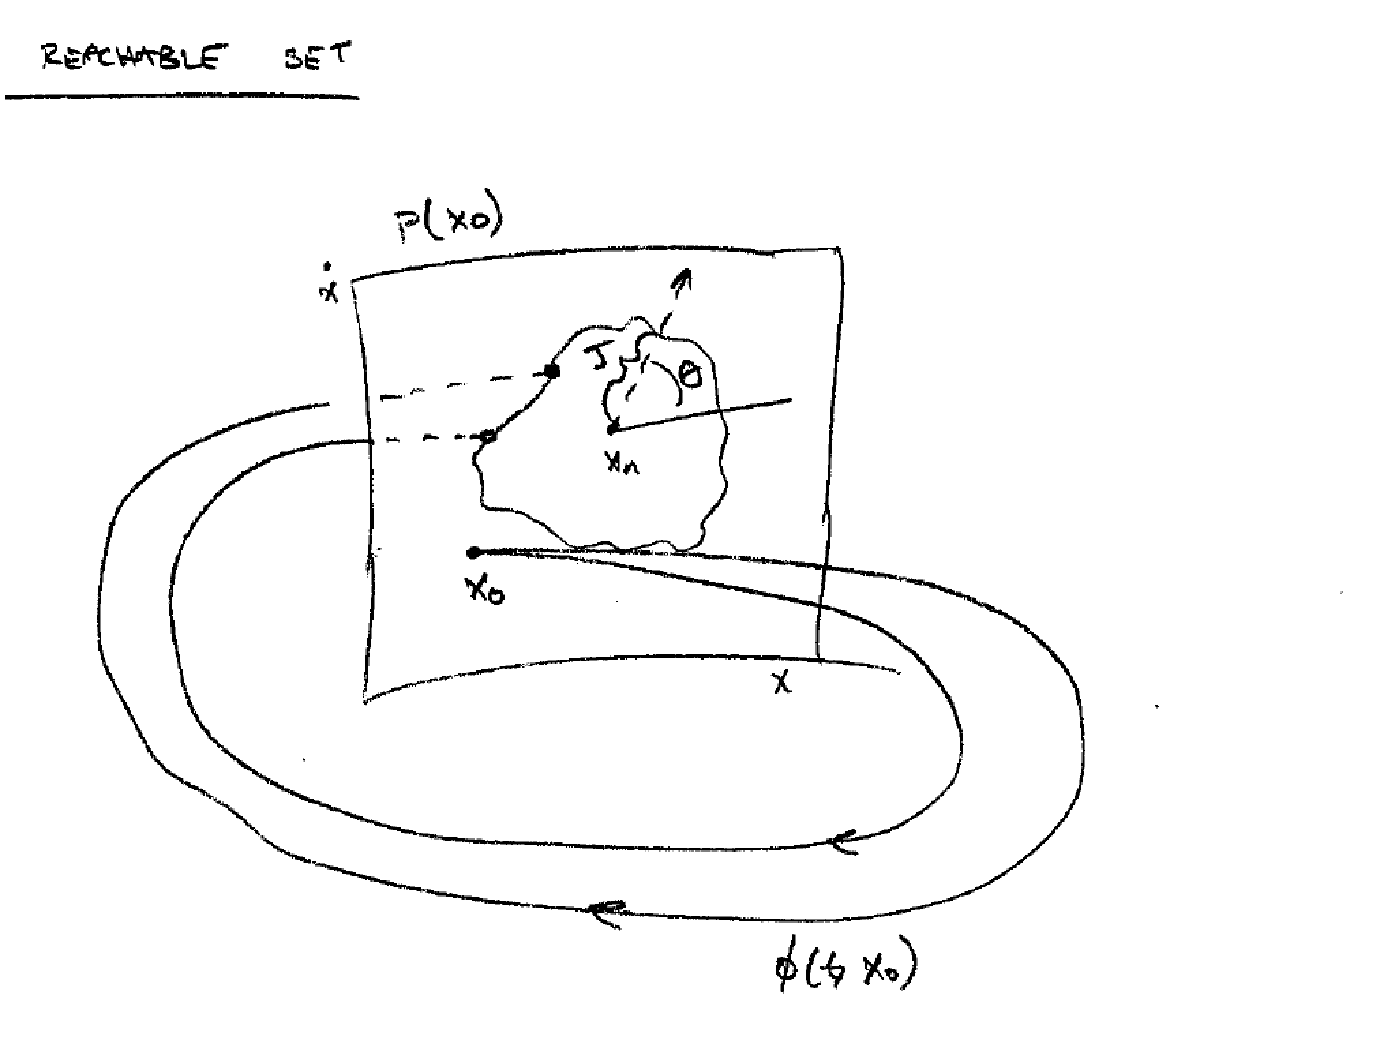
\includegraphics[width=0.5\textwidth]{reachability_set_hand}
        \begin{scaletikzpicturetowidth}{0.6\textwidth}
          \tdplotsetmaincoords{60}{125} % view angle in spherical coordinates
        \begin{tikzpicture}[tdplot_main_coords,
          poincare/.style={opacity=.2,very thick,fill=blue},
          orbit/.style={very thick,black},
          orbit hidden/.style={very thick,dashed},
          grid/.style={very thin,black},
          axis/.style={->,blue,thick},
          reachability/.style={thick,blue},scale=\tikzscale]

        % nodes for the poincare section
        \node[label=above:\(\Sigma\)] (upper_right) at (0,5,5) {};
        \node[] (upper_left) at (0,1,5) {};
        \node[] (lower_left) at (0,1,0) {};
        \node[] (lower_right) at (0,5,0) {};

        % draw poincare section
        \draw[poincare] (upper_right.center) -- (upper_left.center) -- (lower_left.center) -- (lower_right.center) -- (upper_right.center);
        
        % draw a periodic orbit
        \coordinate (center) at (0,0,2);
        \node[label=below:\(\vecbf{x}_n\)] (x0) at (0,3,2) {};
        % \node[label=below:\(\vecbf{x}_n\)] at (x0) {};
        \filldraw (x0) circle (3pt);

        % \tdplotdrawarc[orbit hidden]{(center)}{3}{90}{200}{}{};
        \tdplotdrawarc[orbit,<-]{(center)}{3}{-160}{90}{}{};

        % draw reachability set on the poincare section
        \coordinate (reach) at (0,4.5,2);
        \tdplotsetthetaplanecoords{90}

        \draw[tdplot_rotated_coords,grid] (x0) -- (reach);
        \draw[tdplot_rotated_coords,grid] (x0) -- ++(-45:1.5);

        \tdplotdrawarc[tdplot_rotated_coords,grid]{(x0)}{0.5}{-45}{90}{above}{\(\theta_d\)};

        % draw terminal state on reachability set
        \node[tdplot_rotated_coords,label=above:\(\vecbf{x}_f\)] (xf) at ($ (x0)+(-45:1.5) $) {};
        \filldraw (xf) circle (3pt);

        \node[tdplot_rotated_coords,label=below:\(J\)] at (xf) {};

        \tdplotdrawarc[tdplot_rotated_coords,reachability]{(x0)}{1.5}{0}{360}{}{};
        % place
    \end{tikzpicture}
        \end{scaletikzpicturetowidth}
        \caption{Reachability set on a \Poincare section: Pictorial representation of the reachability set (blue circle) on the \Poincare section, \(\Sigma\). 
            The terminal state, \( x_n\), is the intersection without any control input. 
            Adding a control input allows for the terminal state, \( x_f \), to be displaced by some distance/cost \( J \) as measured on the section.
            We parameterize a specific direction on the section with the angles \( \theta_d\) and seek to maximize the distance between \( x_f \) and \( x_n \).
            Computation of the maximum distance, or reachability, for a variety angles gives a discrete approximation of the reachability set.\label{fig:reachability_set}}
\end{figure}

We define the \Poincare section along the horizontal axis, which is equivalent to the surface \( y = 0 \), and given by
\begin{align}
        \Sigma = \braces{ ( x, \dot{x}) \, | \, y = 0} . 
        \label{eqn:poincare_section}
\end{align}
This is similar to the previous work in determining homoclinic orbits in the three-body problem~\cite{llibre1985,koon2011}.
Previous analytical results have shown that homoclinic orbits intersect transversally in the \( (x, \dot{x} ) \) space on the plane \( y = 0 \).
We seek to compliment these results with the addition of low thrust propulsion to maximize the reachable set on the \Poincare section.
Placing our section at \( y = 0\) ensures that all trajectories will intersect our section.
An optimal control problem is defined by a  cost function
\begin{equation}
        J = -\frac{1}{2} \left( \vc{x}(N) - \vc{x}_{n}(N)\right)^T 
        \left[
        \begin{array}{cccc}
                1 & 0& 0& 0 \\
                 0& 0& 0& 0\\
                 0 & 0 & 1 &0\\
                 0 & 0& 0& 0
        \end{array}
        \right]
        \left( \vc{x}(N) - \vc{x}_{n}(N)\right) = \phi(\vc{x}(N),\vc{x}_n(N)) \, .
        \label{eq:cost}
\end{equation}
The term \( \vc{x}_n(N) \) is the final state of a control-free trajectory while the term \( \vc{x}(N)\) is the final state under the influence of the control input.
Maximization of the distance between \( \vc{x}_n \) and \(\vc{x} \), on the \Poincare section defined in~\cref{eqn:poincare_section} at the terminal time \( t_f = N \), is equivalent to the minimization of \( J \) defined in~\cref{eq:cost}.
The \Poincare section is defined through the use of appropriate terminal constraints given by
\begin{subequations}
\begin{align}
    v_1( \vc{x}(N) ) &= y(N) = 0 \, , \\ 
    v_2 ( \vc{x}(N) )&=  \frac{\dot{x}(N) - \dot{x}_n(N) }{x(N) -x_n(N) } - \tan{\theta_d} = 0\, , \\
         0 &\geq\vc{u}^T \vc{u} - u_{max}^2 \, ,
\end{align}
    \label{eq:constraints}
\end{subequations}
where the angle \( \theta_d\) defines a direction in which we wish to maximize the reachability set on the \Poincare section.
The maximum control thrust magnitude is defined by \( u_{max} \) and is non-dimensionalized by the characteristic units of length, mass, and time.
The goal is to determine the control input \( \vc{u}_k\) such that the cost function~\cref{eq:cost} is minimized subject to the state equations of motion~\cref{eqn:cont_dyn} and constraints~\cref{eq:constraints}.

Application of the Euler-Lagrange equations allows us to derive the necessary conditions for optimality~\cite{bryson1975}.
This results in an optimal control problem and the necessary conditions are given as
\begin{subequations}\label{eq:necc_cond}
\begin{align}
    \dot{\vc{\lambda}} &= - \deriv{H}{\vc{x}}, \\
        0 &=  \deriv{H}{\vc{u}} \, , \label{eqn:control_necc_cond}\\
        0 &= \deriv{\phi}{\vc{x}}^T + \deriv{\vc{v}}{\vc{x}}^T \vc{\beta}  - \vc{\lambda}^T(N) \, ,  
\end{align}
\end{subequations}
where the Hamiltonian \(H\) is defined as
\begin{equation}
        H = \vc{\lambda}^T \vc{f}(\vc{x}, \vc{u}) \, ,
        \label{eq:hamiltonian_opt}
\end{equation}
and \( \vc{\lambda} \in \R^{4 \times 1} \) is the costate and \(\vecbf{\beta} \in \R^{2 \times 1} \) are the additional Lagrange multipliers associated with the terminal constraints in~\cref{eq:constraints}.
The state dynamics are represented by \( \vc{f}(\vc{x}_k, \vc{\lambda}_k ) \) after substituting~\cref{eqn:control_necc_cond} into~\cref{eqn:cont_dyn}.
This indirect optimal control formulation leads to a two point boundary value problem with split boundary conditions. 
By sweeping the angle \( \theta_d \) one can approximate the reachable set on the \Poincare section subject to the bounded control input. 

The optimal control formulation presented in this section results in a \gls{tpbvp}. 
There exist many methods to solve \glspl{tpbvp} such as gradient, quasilinearization, and shooting methods~\cite{bryson1975,kirk2012}.
Shooting methods are common in astrodynamic trajectory design problems and relatively simple to implement.
In the shooting method, initial conditions are varied such that a terminal constraint is satisfied, similar to the way an archer modifies the bow in order to more accurately strike a target. 
Consider the vector of initial conditions, \( \vc{\chi} = \braces{\vc{x}_0, \vc{\lambda}_0}\), which is varied to satisfy some terminal constraints of the form \( \vc{G}(\vc{\chi}) = \braces{\vc{x}_t - \vc{x}_n} = 0 \).
The free variables at the terminal time are computed by propagation of \( \vc{\chi} \) over the selected time horizon. 
At the terminal time, the constraint vector is calculated and if not satisfied \( \vc{\chi}\) is varied.
Rather than numerical integration over the entire time interval, multiple shooting segments the interval into several smaller sub-arcs~\cite{stoer2013}.
This multiple shooting approach incorporates additional interior constraints but reduces the sensitivity of the costates along each sub-arc.
The use of the multiple shooting method reduces the sensitivity of changes in the initial costate at the expense of additional design variables, but has been shown to provide more stable and robust solutions~\cite{ozimek2010a}.

\begin{figure}
        \centering
        \begin{scaletikzpicturetowidth}{1\textwidth}
                \begin{tikzpicture}[scale=\tikzscale]
                    % \draw[help lines] (0,0) grid (20,5) ; %grid

                    \node[label=west:\(\vc{x}\)] (x0m) at (0,5) {};
                    \node[] (x1m) at (5,5) {};
                    \node[] (x2m) at (10,5) {};
                    \node[] (x3m) at (15,5) {};
                    \node[] (xnm) at (20,5) {};

                    \node[label=below:\(k_0\)] (t0) at (0,0) {};
                    \node[label=below:\(k_1\)] (t1) at (5,0) {};
                    \node[label=below:\(k_2\)] (t2) at (10,0) {};
                    \node[label=below:\(k_{n-1}\)] (t3) at (15,0) {};
                    \node[label=below:\(k_n\)] (tn) at (20,0) {};

                    % nodes for each subsegment
                    \node[label=left:\(\vc{x}_0\)] (x0) at (0,1) {\pgfuseplotmark{*}};
                    \node[label=below left:\(\vc{\lambda}_0\)] at (x0) {};

                    \node[label=right:\(\vc{x}_1^{-}\)] (x1minus) at (5,2) {\pgfuseplotmark{*}};
                    \node[label=below right:\(\vc{\lambda}_1^{-}\)] at (x1minus) {};

                    \node[label=above left:\(\vc{x}_1^{+}\)] (x1plus) at (5,3) {\pgfuseplotmark{o}};
                    \node[label=left:\(\vc{\lambda}_1^{+}\)] at (x1plus) {};

                    \node[label=right:\(\vc{x}_2^{-}\)] (x2minus) at (10,2) {\pgfuseplotmark{*}};
                    \node[label=below right:\(\vc{\lambda}_2^{-}\)] at (x2minus) {};

                    \node[label=above left:\(\vc{x}_2^{+}\)] (x2plus) at (10,3) {\pgfuseplotmark{o}};
                    \node[label=left:\(\vc{\lambda}_2^{+}\)] at (x2plus) {};

                    \node[label=right:\(\vc{x}_{n-1}^{-}\)] (x3minus) at (15,2) {\pgfuseplotmark{*}};
                    \node[label=below right:\(\vc{\lambda}_{n-1}^{-}\)] at (x3minus) {};

                    \node[label=above left:\(\vc{x}_{n-1}^{+}\)] (x3plus) at (15,3) {\pgfuseplotmark{o}};
                    \node[label=left:\(\vc{\lambda}_{n-1}^{+}\)] at (x3plus) {};

                    \node[label=right:\(\vc{x}_n\)] (xnminus) at (20,3) {\pgfuseplotmark{*}};
                    \node[label=below right:\(\vc{\lambda}_n\)] at (xnminus) {};
                    % draw axes
                    \draw [<->,thick] (tn.center) -- (t0.center) -- (x0m.center);

                    % draw segement dividers
                    \draw [dashed,thick] (t1.center) -- (x1m.center);
                    \draw [dashed,thick] (t2.center) -- (x2m.center);
                    \draw [dashed,thick] (t3.center) -- (x3m.center);
                    \draw [dashed,thick] (tn.center) -- (xnm.center);

                    % draw markers at each subsegment

                    % draw the subsegments
                    \draw [->] (x0.center) to [bend left=30] (x1minus.center);
                    \draw [->] (x1plus.center) to [bend left=30] (x2minus.center);
                    % dotted lines here
                    \draw[decorate sep={1mm}{5mm},fill] (x2plus.east) to [bend left=10] (x3minus.west);

                    \draw [->] (x3plus.center) to [bend left=30] (xnminus.center);
                \end{tikzpicture}
        \end{scaletikzpicturetowidth}
        \caption{Schematic diagram of the multiple shooting method:
        The complete trajectory is split into a number of sub-segments, and additional interior constraints are included to ensure state and costate continuity.
    Splitting the optimal trajectory into short segments reduces the sensitivity of terminal states to variations of the initial states.\label{fig:multiple shooting}}
\end{figure}

In~\cref{fig:multiple shooting}, we show a schematic representation of the multiple shooting procedure.
We split the optimal control horizon into equal length subsegments such that the length of each segment is \( \frac{k}{n} \), where \( k, n \) are the total number of steps and number of stages, respectively.
Similarly, we divide the state and costate trajectories into \( n \) equal segments. 
To ensure continuity, additional interior constraints are incorporated as
\begin{align}\label{eq:interior_constraints}
        \vc{x}_1^{-} - \vc{x}_1^{+} &= 0 , \nonumber\\ 
        \vc{\lambda}_1^{-} - \vc{\lambda}_1^{+} &= 0 , \nonumber\\
        \vc{x}_2^{-} - \vc{x}_2^{+} &= 0 , \nonumber\\ 
        \vc{\lambda}_2^{-} - \vc{\lambda}_2^{+} &= 0 , \nonumber\\
        &\vdots \nonumber \nonumber\\
        \vc{x}_{n-1}^{-} - \vc{x}_{n-1}^{+} &= 0 , \nonumber\\ 
        \vc{\lambda}_{n-1}^{-} - \vc{\lambda}_{n-1}^{+} &= 0.
\end{align}
Using the multiple shooting method reduces the sensitivity of the terminal states, \( \vc{x}_i^{+}, \vc{\lambda}_i^{+}\), to variations of the initial states, \(\vc{x}_{i-1}^{-}, \vc{\lambda}_{i-1}^{-}\).
As a result, the design vector \( \vc{\chi} \) is augmented with the additional interior initial conditions, \( \vc{x}_i^{-}, \vc{\lambda}^{-}\).
Similarly, the constraint vector is augmented with the additional interior constraints defined in~\cref{eq:interior_constraints}.
Based on experimentation, we use four stages in our multiple shooting method.
This provided the best performance and convergence stability while minimizing the difficulties in additional interior constraints.
The multiple shooting algorithm now varies the design vector \( \vc{\chi}\) to ensure that the constraints in \( \vc{G}(\vc{\chi}) \) are satisfied.
In this work, we use the Matlab nonlinear solver \texttt{fsolve} to solve the system of nonlinear equations defined by the multiple shooting algorithm with a convergence tolerance of \num{1e-5}.
Within \texttt{fsolve}, we use the trust-region dogleg solver which makes use of the Powell dogleg procedure for computing a step direction and magnitude to minimize successive iterations of the solver.
The numerical results are specific to the choice of nonlinear solver, and different tolerances or software tools may result in slight changes.

% TODO Add numerical examples of the three-body problem
\section{Numerical Examples of Transfers using Reachability Sets}\label{sec:simulation}
We present two numerical simulations in the Earth-Moon system to demonstrate the transfer procedure.
These simulations enable the spacecraft to depart from the natural dynamics through the use of low-thrust propulsion.
The reachability set on the \Poincare section allows for a straightforward method of determining transfer opportunities.
The first example is a transfer from a periodic orbit of the \( L_1 \) Lagrange point to a fixed orbit of the moon.
This example uses a single iteration of the reachable set computation in the design of the transfer.
The second example is a transfer from geostationary orbit of the Earth to a period orbit of \( L_1 \). 
This examples demonstrates the ability to extend the reachability process to multiple iterations, to allow for a much larger and more general transfer.
With both examples it is possible to depart from the vicinity of the Earth to a Moon orbit via a series of reachable sets defined on \Poincare sections.
The numerical examples presented in this section satisfy the necessary conditions for local optimality and obtaining a globally optimal solution is considered beyond the scope of this paper.
Next, the results are extended from the planar problem to three dimensions with a simulation about asteroid 4769 Castlia.
This numerical examples demonstrates the extension of the method to the more complicated dynamic enviornment around an asteroid.

\subsection{Three Body Examples}

\paragraph{Periodic Orbit Transfer}
The first objective is to design a transfer trajectory from a planar periodic orbit about the \( L_1\) Lagrange point to a bounded orbit in the vicinity of the Moon.
The target region is created by choosing an initial condition of \( x_0 = \begin{bmatrix}1.05 & 0 & 0 & 0.35 \end{bmatrix}^T \) with \( \mu = 0.0125 \).
The target set is propagated over a period of \( t = \num{20} \) in non-dimensional units which corresponds to approximately \num{1.5} years.
\begin{figure}[htbp]
   \centering
   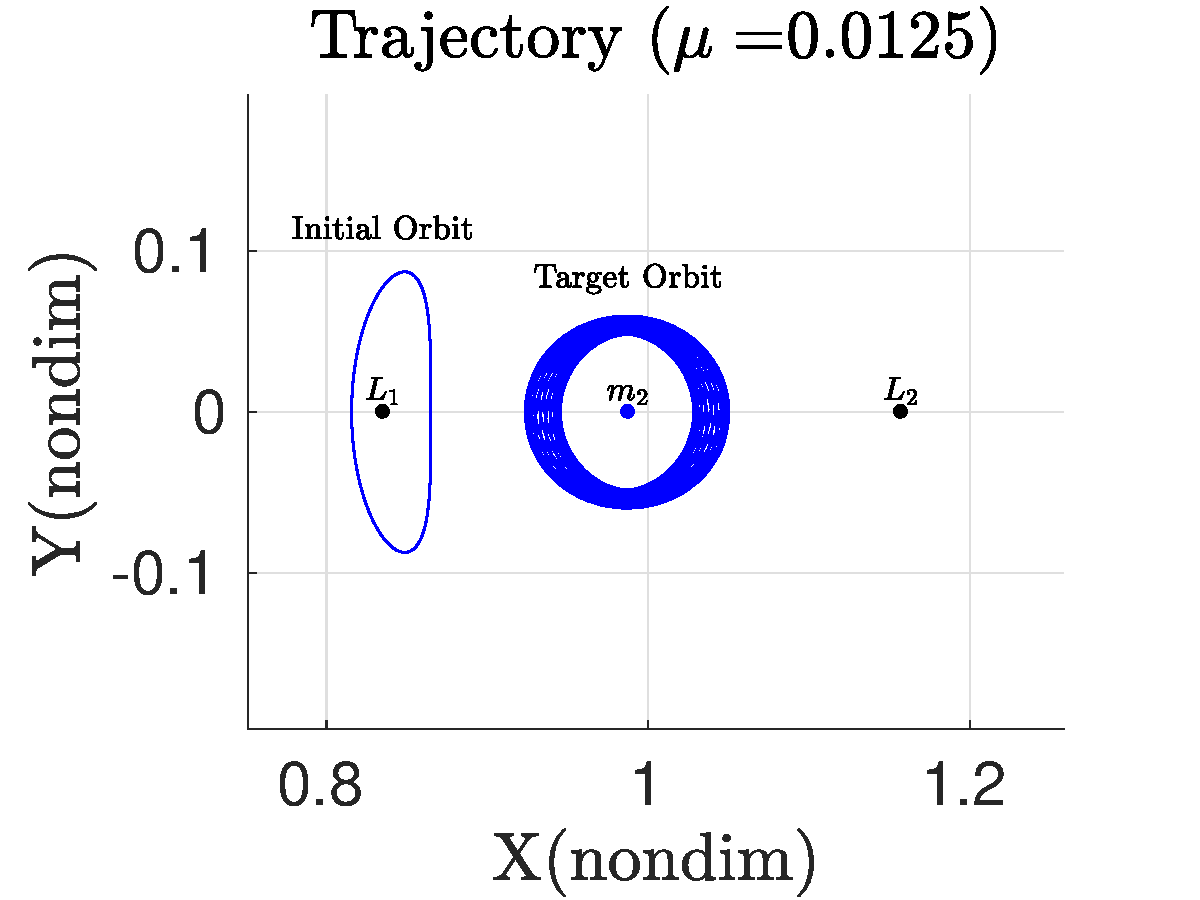
\includegraphics[width=0.5\textwidth]{figures/2017_JAS/moon_orbit.pdf} % requires the graphicx package
   \caption{\(L_1\) periodic orbit transfer to orbit of the Moon: Example scenario demonstrating the initial and target orbit.
   Without the low-thrust propulsion, the spacecraft is constrained to the initial periodic orbit. 
   We determine the reachability set to find a transfer trajectory to the target orbit about the moon.}
   \label{fig:moon_orbit}
\end{figure}
\Cref{fig:moon_orbit} shows that the target set remains in the vicinity of the Moon, or \( m_2\), in the rotating reference frame. 
This type of orbit would be useful for a variety of mission scenarios.
For example, a series of communication satellites could be placed in this type of orbit. 
The bounded trajectories of the vehicles and constant line of sight to both the Moon and the Earth would allow for constant communication for future manned missions and potential habitats.
The initial set is a planar periodic orbit about \( L_1\), which is generated using the process of differential correction of a linear approximation~\cite{koon2011}.

% invariant manifold transfer
As a source for comparison, the method of using invariant manifolds, introduced in~\cite{koon2011}, is implemented.
As described in~\cref{sec:invariant_manifold}, these invariant manifolds are the set of trajectories that either asymptotically arrive or depart the periodic orbit. 
We generate the unstable manifold associated with the initial planar periodic orbit.
We numerically propagate the unstable manifold forward in time until the trajectories intersect the \Poincare section \( y = 0 \).
\Cref{fig:manifold_trajectory} shows the unstable invariant manifold generated from the initial \( L_1\) periodic orbit. 
The blue points in~\cref{fig:manifold_poincare} are the intersections of the target Moon orbit and the \Poincare section.
The two circular regions are the ascending (right) and descending (left) intersections of the target orbit and \Poincare section.
The green points in~\cref{fig:manifold_poincare} are intersections of the unstable manifold from~\cref{fig:manifold_trajectory} with the \Poincare section \( y = 0 \).
Only a single branch of the invariant manifold intersects with the ascending region of the target orbit.
There are no intersections of the invariant manifold with the descending region of the target orbit.
The numerical values associated with the green points denote the required time of flight along the invariant manifold in non-dimensional units.
The required travel time for a transfer using the unstable invariant manifold is  approximately \( t_f \approx 3.1\) non-dimensional time units.
\begin{figure} 
        \centering 
        \begin{subfigure}[htbp]{0.5\textwidth} 
            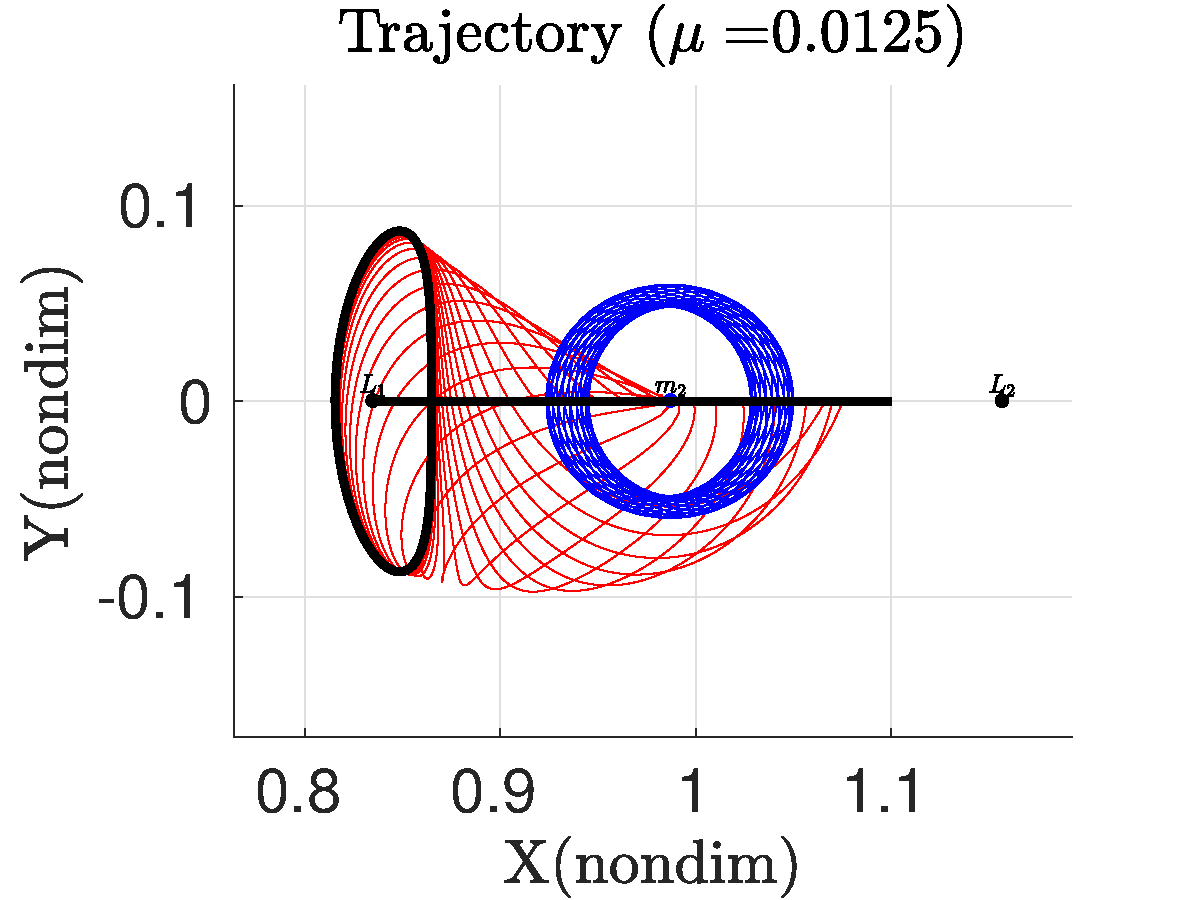
\includegraphics[width=\textwidth]{figures/2017_JAS/manifold_trajectory} 
                \caption{Position space view of invariant manifold} \label{fig:manifold_trajectory} 
        \end{subfigure}~ %
        \begin{subfigure}[htbp]{0.5\textwidth} 
            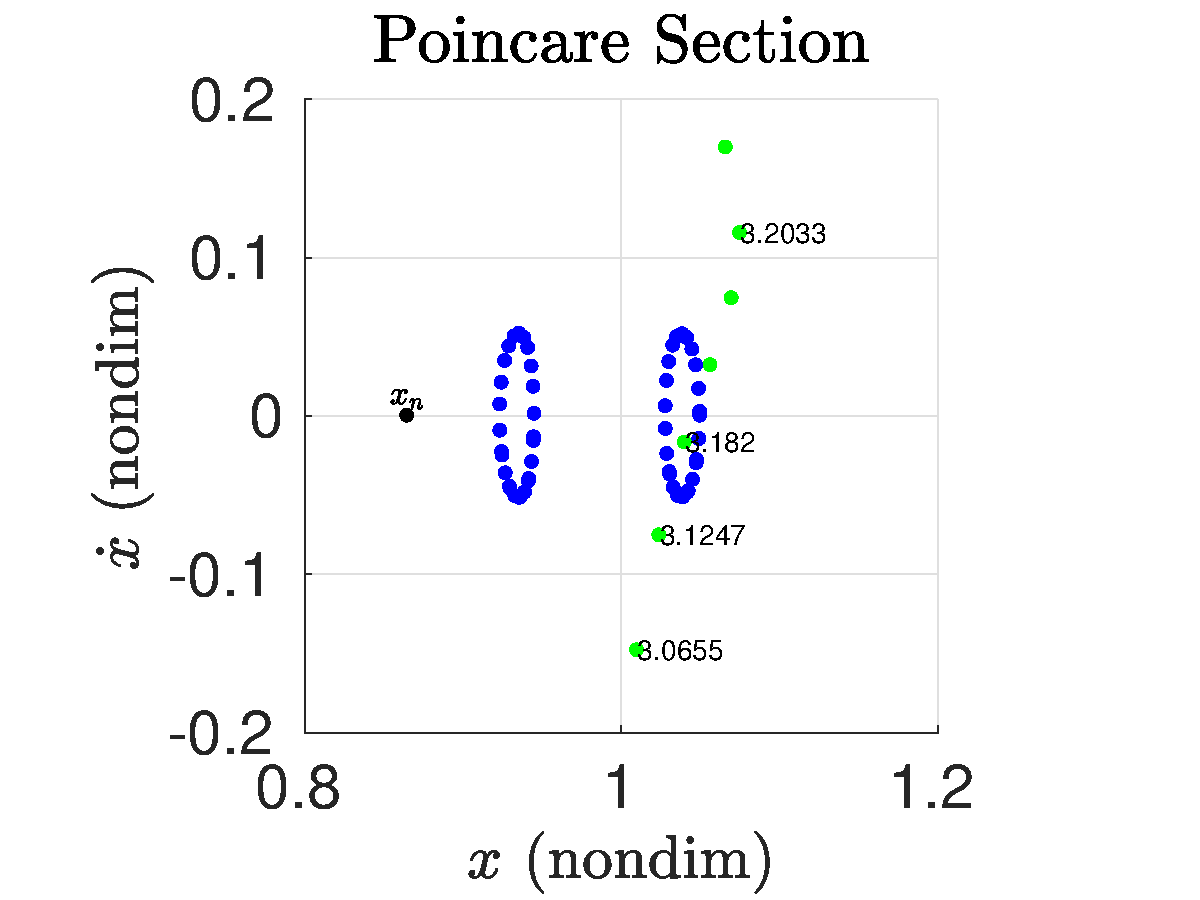
\includegraphics[width=\textwidth]{figures/2017_JAS/manifold_poincare} 
                \caption{\Poincare intersection of invariant manifold (green), target orbit (blue) and the initial orbit (black)} \label{fig:manifold_poincare} 
        \end{subfigure} 
        \caption{Invariant manifold transfer: An example transfer using the invariant manifolds is shown in both the position and \Poincare spaces.
        The control free transfer from the initial periodic orbit to the target orbit result in a long time of flight. 
    In addition, the manifold only intersects the target orbit on the ascending or far side of the moon.}
        \label{fig:invariant_manifold_transfer} 
\end{figure}

Next, we determine the reachability set with addition of a low-thrust control input over a fixed time horizon.
In~\cref{fig:varying_tf_reachability_sets}, we demonstrate the effect of variations in the choice of maximum control bound and terminal time.
While~\cref{sssec:periodic_orbit_transfer} show a specific example of a transfer design process using the intersection of the reachability set on the \Poincare section.
The analysis presented in the following sections define a maximum magnitude of the thrust as \( u_{m} \) and assume that the trust can be directed arbitrarily within the plane. 
This model is representative of many spacecraft which have a body fixed thruster and attitude control system.
Assuming a fully actuated spacecraft model allows us to decouple the translation and rotational dynamics of the spacecraft.

\paragraph{Reachability Set on the \Poincare section}
From the initial state on the periodic orbit, a series of optimal trajectories are generated to determine the reachable set.
The multiple shooting approach is implemented to solve the optimal control problem. 
We divide the time horizon into two equal length segments. 
The state trajectory is initialized using the free trajectory of the periodic orbit. 
Similarly, the costate trajectory is initialized from an initial guess of \( \vc{\lambda}_0 = \begin{bmatrix} -1 & -1 & -1 & -1\end{bmatrix}^T\) and propagated using the system dynamics.
This results in the initial guess of the design vector \( \vc{\chi} = \begin{bmatrix} \vc{\lambda}_0 & \vc{x}_1^{-} & \vc{\lambda}_1^{-} & \vc{\beta} \end{bmatrix}^T\).
This design vector is then varied to ensure that the necessary conditions of optimality and the interior point constraints are satisfied. 
\Cref{tab:varying_tf} shows the range of terminal times, \( t_f \), and maximum control bound, \( u_m \), which are used to investigate their effect on the subsequent reachable set on the \Poincare section.
\begin{table}
    \centering
    \begin{tabular}{ll}  
        \toprule
        \(t_f\) & \( u_m \) \\
        \midrule
        1.24 & 0.05 \\
        1.30 & 0.25 \\
        1.37 & 0.5 \\
        1.44 & \\
        \bottomrule
    \end{tabular}
    \caption{Combinations for \( t_f \) and \( u_m\) used to generate the reachability sets in~\cref{fig:varying_tf_reachability_sets}~\label{tab:varying_tf}}
\end{table}

The angle \( \theta_d\) in~\cref{eq:constraints} is varied to select a different direction along the \Poincare section to maximize.
We discretely vary the angle over the range \( \ang{0} \leq \theta_d < \ang{360} \) to approximate the reachability set of the spacecraft.
Choosing a new angle \( \theta_d \) corresponds to a different direction as well as a new optimal control problem which is again solved using the multiple shooting approach laid out previously.
Each optimal control solution, corresponding to a discrete value of \( \theta_d \), is solved using \texttt{fsolve} as described earlier. 
Each solution on the reachability set is computed in approximately \SI{2}{\minute} on a desktop computer using an \SI{3.4}{\giga\hertz} Intel i7-3700.
The intersection of the optimal trajectories as well as those of the target Moon orbit with the \Poincare section are shown in~\cref{fig:varying_tf_reachability_sets}.

\begin{figure}
    \subcaptionbox{Position space view of reachability sets\label{fig:varying_tf_trajectory}}{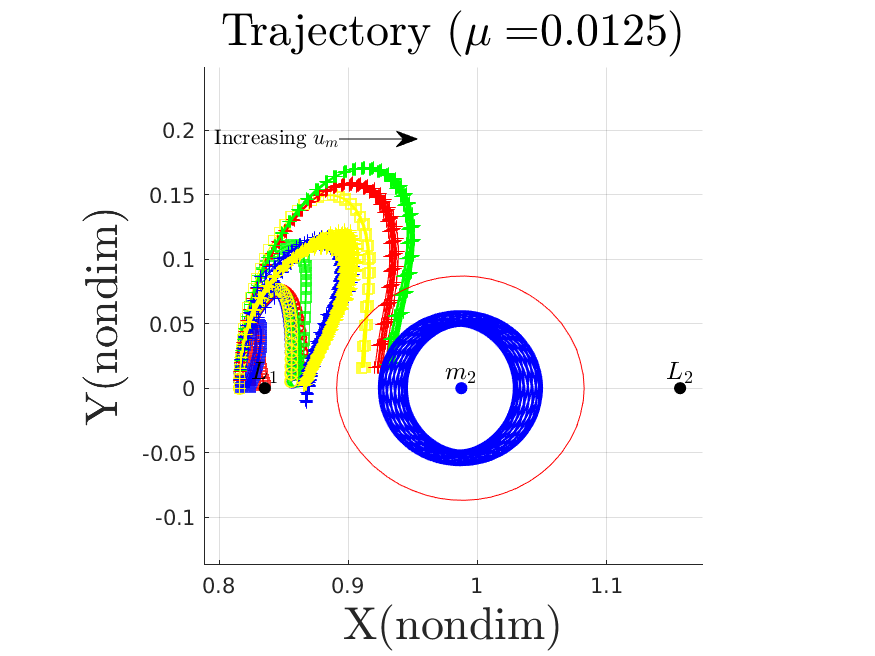
\includegraphics[width=0.5\textwidth]{figures/2017_JAS/trajectory_varying_um.pdf}}~
    \subcaptionbox{\Poincare section view of reachability sets\label{fig:varying_tf_poincare}}{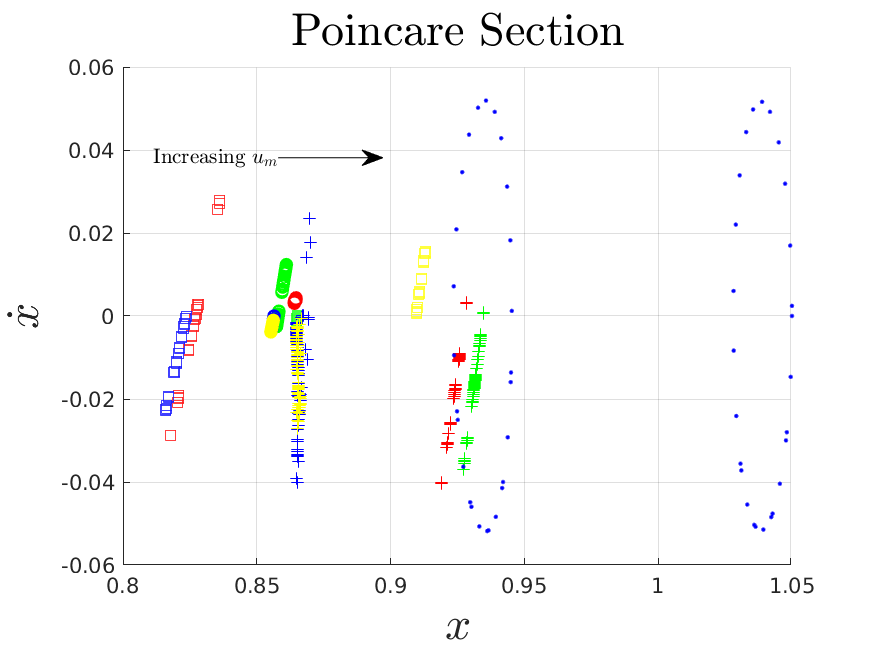
\includegraphics[width=0.5\textwidth]{figures/2017_JAS/poincare_section_varying_um.pdf}}
    \caption{Variation of \( t_f \) and \( u_m\) on the reachability set. 
        Colors, \braces{\text{red}, \text{blue}, \text{green}, \text{yellow}}, are used note increasing \( t_f\) while markers, \braces{\text{circle}, \text{square}, \text{cross}}, are used to denote increasing \(u_m\).
    Increasing the maximum control bound has a large effect and enables the reachability set to intersect the target manifold. 
    Increases in \(t_f\) are less critical and have minimal impact on the distribution of the reachability set on the \Poincare section.~\label{fig:varying_tf_reachability_sets}}
\end{figure}

\Cref{fig:varying_tf_reachability_sets} shows the reachabilty set for twelve combinations of \(t_f\) and \( u_m\) listed in~\cref{tab:varying_tf}.
With a small maximum control bound, \( u_m = \num{0.05} \) shown using square markers, the reachable set is not dramatically changed from that of the no control solution.
The reachable set is denoted using square markers on the left most portion of \cref{fig:varying_tf_poincare}.
Variations of \( t_f\) are indicated using different colors and also demonstrate that this parameters has a smaller impact than changes in \( u_m \).
Increasing the control bound to \( u_m = \num{0.25} \) and \( u_m = \num{0.5} \) shows that the reachable set progressively approaches the target set.

The reachable sets presented in~\cref{fig:varying_tf_reachability_sets} are highly dependent on the initial condition, terminal time, and maximum control bound. 
This example demonstrates that increasing the \( u_m \) results in a larger displacement between the controlled and uncontrolled trajectories.
The reachable set is enlarged from a single point, as shown in~\cref{fig:manifold_poincare} by the black point, to a larger region as shown in~\cref{fig:varying_tf_poincare}.
The choice of \( u_m\), \( t_f \) and initial condition all combine to change the resulting reachability set. 

\paragraph{Transfer to Periodic Orbit}~\label{sssec:periodic_orbit_transfer}
% reachable set transfer
Here we use the results of the preceding section to demonstrate one specific example of a transfer designed using the reachability set.
The acceleration limit is chosen as  \( u_{max} = 0.75 \approx \SI{2}{\milli\meter\per\second\squared} \) in the Earth-Moon system.
Assuming a fixed spacecraft mass of \SI{500}{\kilo\gram}, this model defines a maximum thrust of approximately \SI{1}{\newton}.
Currently, the NASA NEXT xenon thruster is able to provide approximately \SI{0.25}{\newton} of thrust, and a cluster of such engines could be used to provide the desired thrust used in this work~\cite{schmidt2008}.
The trajectories are generated from a fixed initial state of \( \vc{x}_0 = \begin{bmatrix}0.8156 & 0 & 0 & 0.1922 \end{bmatrix}^T \) over a fixed time span of \( t_f = 1.4 \).
This initial state lies on the initial periodic orbit and the time of flight is equivalent to one half period of the initial periodic orbit. 

% discuss reachability set computation
The optimal trajectories, under the influence of the control input \( \vc{u} \), are plotted in red in~\cref{fig:reach_trajectory}.
Initially, the spacecraft is assumed to lie on the periodic orbit.
As a result, the intersection of this periodic orbit with the \Poincare section are two points corresponding to the two crossing of the orbit.
We show the control-free intersection, \( \vc{x}_n \), of the periodic orbit on the \Poincare section in~\cref{fig:manifold_poincare,fig:poincare_compare}
The use of the continuous low thrust propulsion expands the reachable set to region bounded by the red markers in~\cref{fig:poincare_compare}.
The reachable set is an ellipsoidal region with a major axis aligned along \( \theta \approx \ang{70} \) as compared to a fixed point without any control input.
\begin{figure} 
        \centering 
        \begin{subfigure}[htbp]{0.5\textwidth} 
            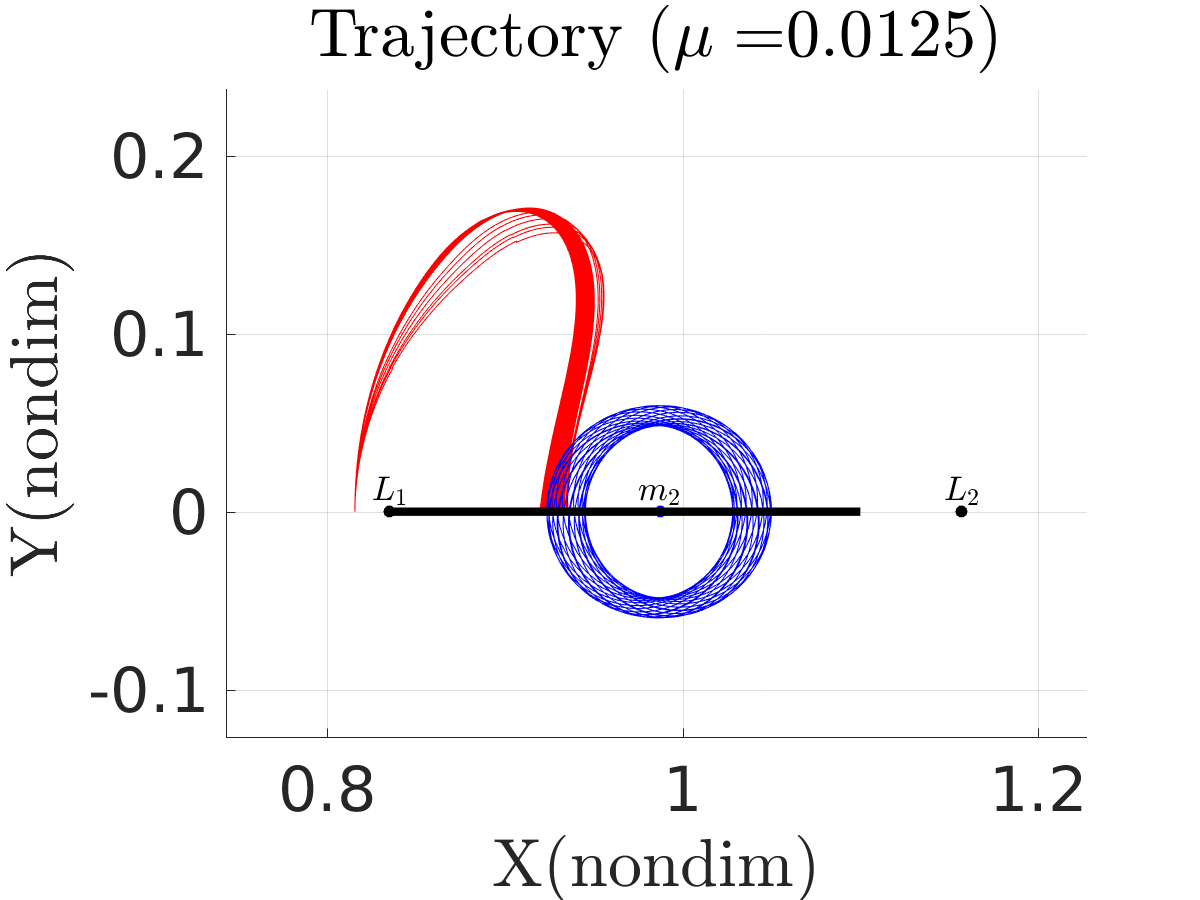
\includegraphics[width=\textwidth]{figures/2017_JAS/reach_trajectory} 
                \caption{Position space view of reachability set} \label{fig:reach_trajectory} 
        \end{subfigure}~ %add desired spacing between images, e. g. ~, \quad, \qquad, \hfill etc. %(or a blank line to force the subfigure onto a new line) 
        \begin{subfigure}[htbp]{0.5\textwidth} 
            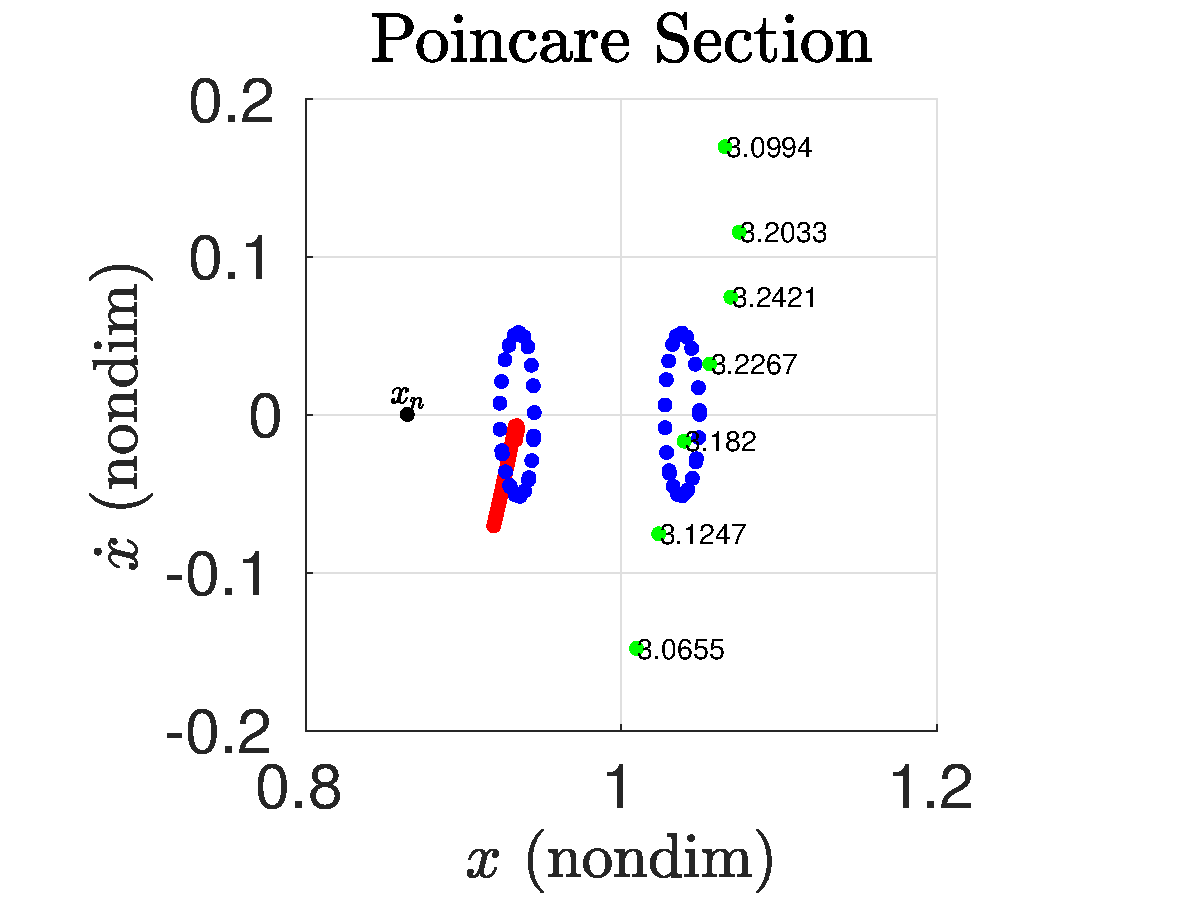
\includegraphics[width=\textwidth]{figures/2017_JAS/poincare_compare} 
                \caption{\Poincare section view of reachability set} \label{fig:poincare_compare} 
        \end{subfigure} %add desired spacing between images, e. g. ~, \quad, \qquad, \hfill etc. %(or a blank line to force the subfigure onto a new line) 
                
        \begin{subfigure}[htbp]{0.5\textwidth} 
            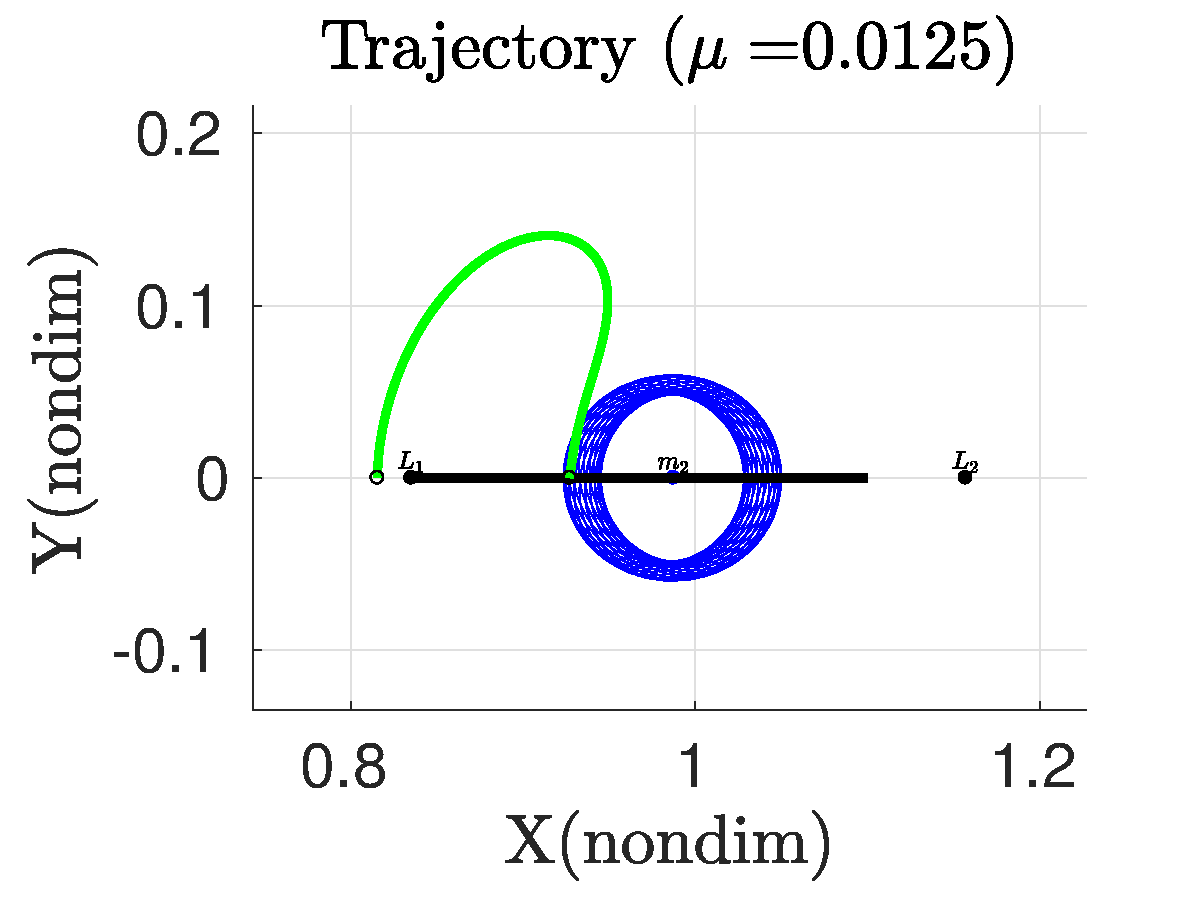
\includegraphics[width=\textwidth]{figures/2017_JAS/reach_transfer} 
                \caption{Transfer trajectory selected from reachability set viewed in the position space} \label{fig:reach_transfer} 
        \end{subfigure}~ 
        \begin{subfigure}[htbp]{0.5\textwidth} 
            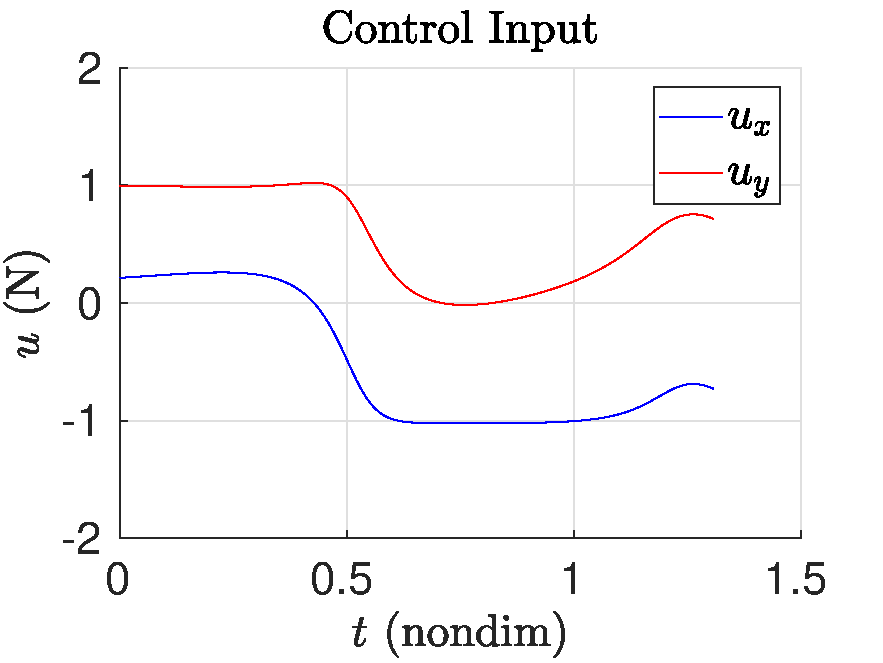
\includegraphics[width=\textwidth]{figures/2017_JAS/control_input_l1} 
                \caption{Control input for the selected transfer trajectory} \label{fig:control_l1} 
        \end{subfigure}~

        \begin{subfigure}[htbp]{0.5\textwidth} 
            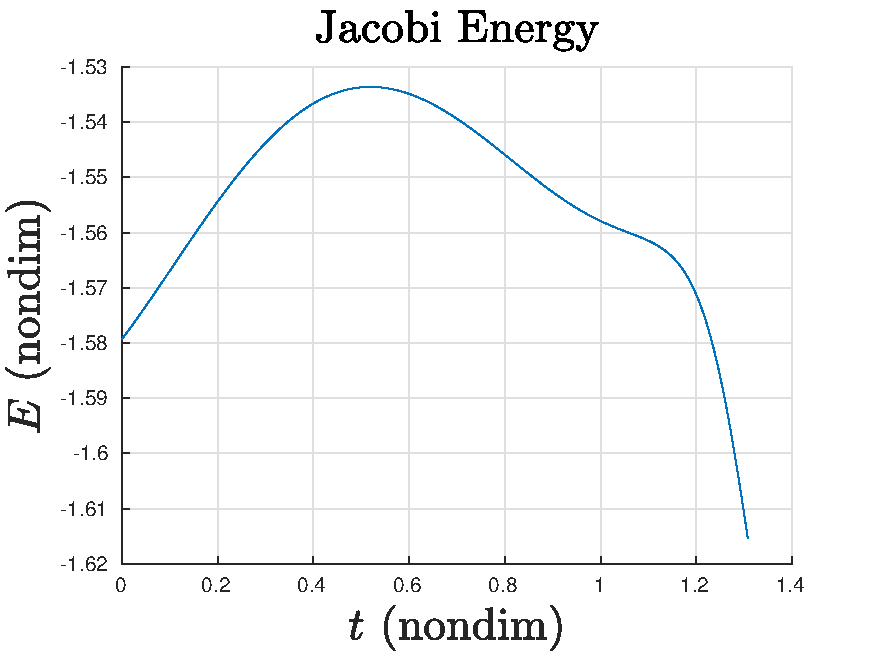
\includegraphics[width=\textwidth, keepaspectratio]{figures/2017_JAS/jacobi.pdf} 
            \caption{Jacobi Energy over transfer \label{fig:jacobi_l1}} 
        \end{subfigure} 

        \caption{\( L_1 \) Reachability set transfer: The low thrust propulsion is used to approximate the reachability set starting from the initial periodic orbit over a fixed time horizon.
            The reachability set is shown in~\cref{fig:reach_trajectory,fig:poincare_compare} in both the position and \Poincare space respectively.
            From this reachability set we chose a trajectory which intersects the target orbit and it is shown in~\cref{fig:reach_transfer}.
        The optimal control to achieve this transfer is shown in~\cref{fig:control_l1}.}
        \label{fig:reachability_set_transfer} 
\end{figure}

% generate the optimal transfer
\Cref{fig:poincare_compare} shows that the reachable set and those of the descending target region intersect.
As both regions are discretely approximated a linear interpolation is used to determine the exact intersection state on the \Poincare section.
This intersection generates a partial target state of \( x_t \text{ and } \dot{x}_t \).
Using the energy level of the target region, defined by~\cref{eq:jacobi}, and the intersection state we can calculate the final component \( \dot{y} \). 
This results in a complete target state \( \vecbf{x}_t \) which lies on the reachable set and on the target orbit. 
A final optimal trajectory is generated such that the \( \vecbf{x}(N) = \vecbf{x}_t \).
This transfer trajectory is denoted by the green path in~\cref{fig:reach_transfer}.
The optimal control input is shown in~\cref{fig:control_l1}. 
The spacecraft achieves the desired target while satisfying the bounded control input.
The Jacobi energy integral, computed using~\cref{eq:jacobi}, is shown in~\cref{fig:jacobi_l1}.
\Cref{fig:jacobi_l1} shows that the vehicle begins with an energy level equal to the periodic orbit and arrives at the target orbit with the appropriate energy.
The first half of the transfer is associated with and increase in energy as the control is used to transition towards the target orbit which is followed by a energy decrease to the target orbit.
This roughly corresponds with the expected optimal solution of a bang-coast-bang type orbital transfer~\cite{kirk2012}.
Convergence statistics associated for this transfer are shown in~\cref{tab:l1_transfer_stats}.
\begin{table}
    \centering
    \begin{tabular}{llr}  
        \toprule
        Metric    & Value \\
        \midrule
        \texttt{fsolve} objective      & \num{6.03e-15}      \\
        \texttt{fsolve} major iterations       & \num{9}      \\
        \texttt{fsolve} first order optimality & \num{1.88e-13} \\
        Optimal cost       & \num{2.09e-31}      \\
        Execution time & \SI{1.49}{\second}       \\
        \bottomrule

    \end{tabular}
    \caption{Convergence statistics for the periodic orbit transfer\label{tab:l1_transfer_stats}}
\end{table}

% compare the invariant manifold method and reachability set
A transfer along the invariant manifold requires on average \( t_f \approx 3.1 \) as compared to \( t_f \approx 1.4 \) for a transfer using low thrust propulsion and the reachable set.
This long time of flight is typical of transfers using invariant manifolds.
The unstable invariant manifold traverses a large region of the phase space and is dependent on the system dynamics. 
In addition, the invariant manifolds asymptotically arrive and depart from the periodic orbit. 
As a result, it may take an arbitrarily long period of time to depart from the vicinity of the periodic orbit.
In addition, only a small portion of the invariant manifold intersects with the target Moon orbit.
In contrast, the low thrust control input we are able to enlarge the reachability set from a single point, \( x_n\) associated with the periodic orbit, to a larger ellipsoidal region shown in red in~\cref{fig:poincare_compare}.
This achieves an intersection with the target orbit with a much lower time of flight as compared to the invariant manifold method.
In addition, by generating the reachability set we are able to compute the required control input to exactly intersect the target orbit.
This avoids having to compute and accomplish a secondary impulsive maneuver to transition from the invariant manifold to the target orbit.
%Since The intersection on the \Poincare section only shows that the \( x \text{ and } \dot{x} \) components intersect.
%An additional instantaneous \( \Delta V \) would be required to transfer from the invariant manifold to the target.

\paragraph{Geostationary Orbit Transfer}
\subsection{4769 Castalia Examples}
